\chapter{Взаимодействие h-BN/Co(0001) с молекулярным кислородом} \label{chapt3}

Теоретические исследования показывают, что взаимодействие монослоя гексагонального 
нитрида бора с кислородом приводит к изменению электронных и магнитных
свойств материала~\cite{Ataca2010,Zhou2010}. Важным обстоятельством является то, каким именно образом кислород
вступает во взаимодействие с ML h-BN, а именно: встраиваются атомы кислорода в решетку 
h-BN, или интеркалируют под монослой, не образуя связей с ним, или же являются 
адатомами на поверхности монослоя. Таким образом, в данной работе был 
исследован механизм взаимодействия молекулярного кислорода с монослоем h-BN, выращенного на 
поверхности кобальта Co(0001). Посредством серии экспериментов на Российско-Германском
канале вывода СИ синхротрона BESSY II в Берлине были получены экспериментальные 
данные XPS, NEXAFS а так же LEED. Результаты и выводы по полученным данным 
представленны в данной работе.

\section{Характеристика структуры образца}

После формирования гексагонального нитрида бора на поверхности кобальта, для контроля
качества  поверхности, была получена картина дифракции медленных электронов
рис.~\ref{pic:LEED}. Постоянные решеток Co(0001) и h-BN практически  
\begin{figure}[!ht]
\center{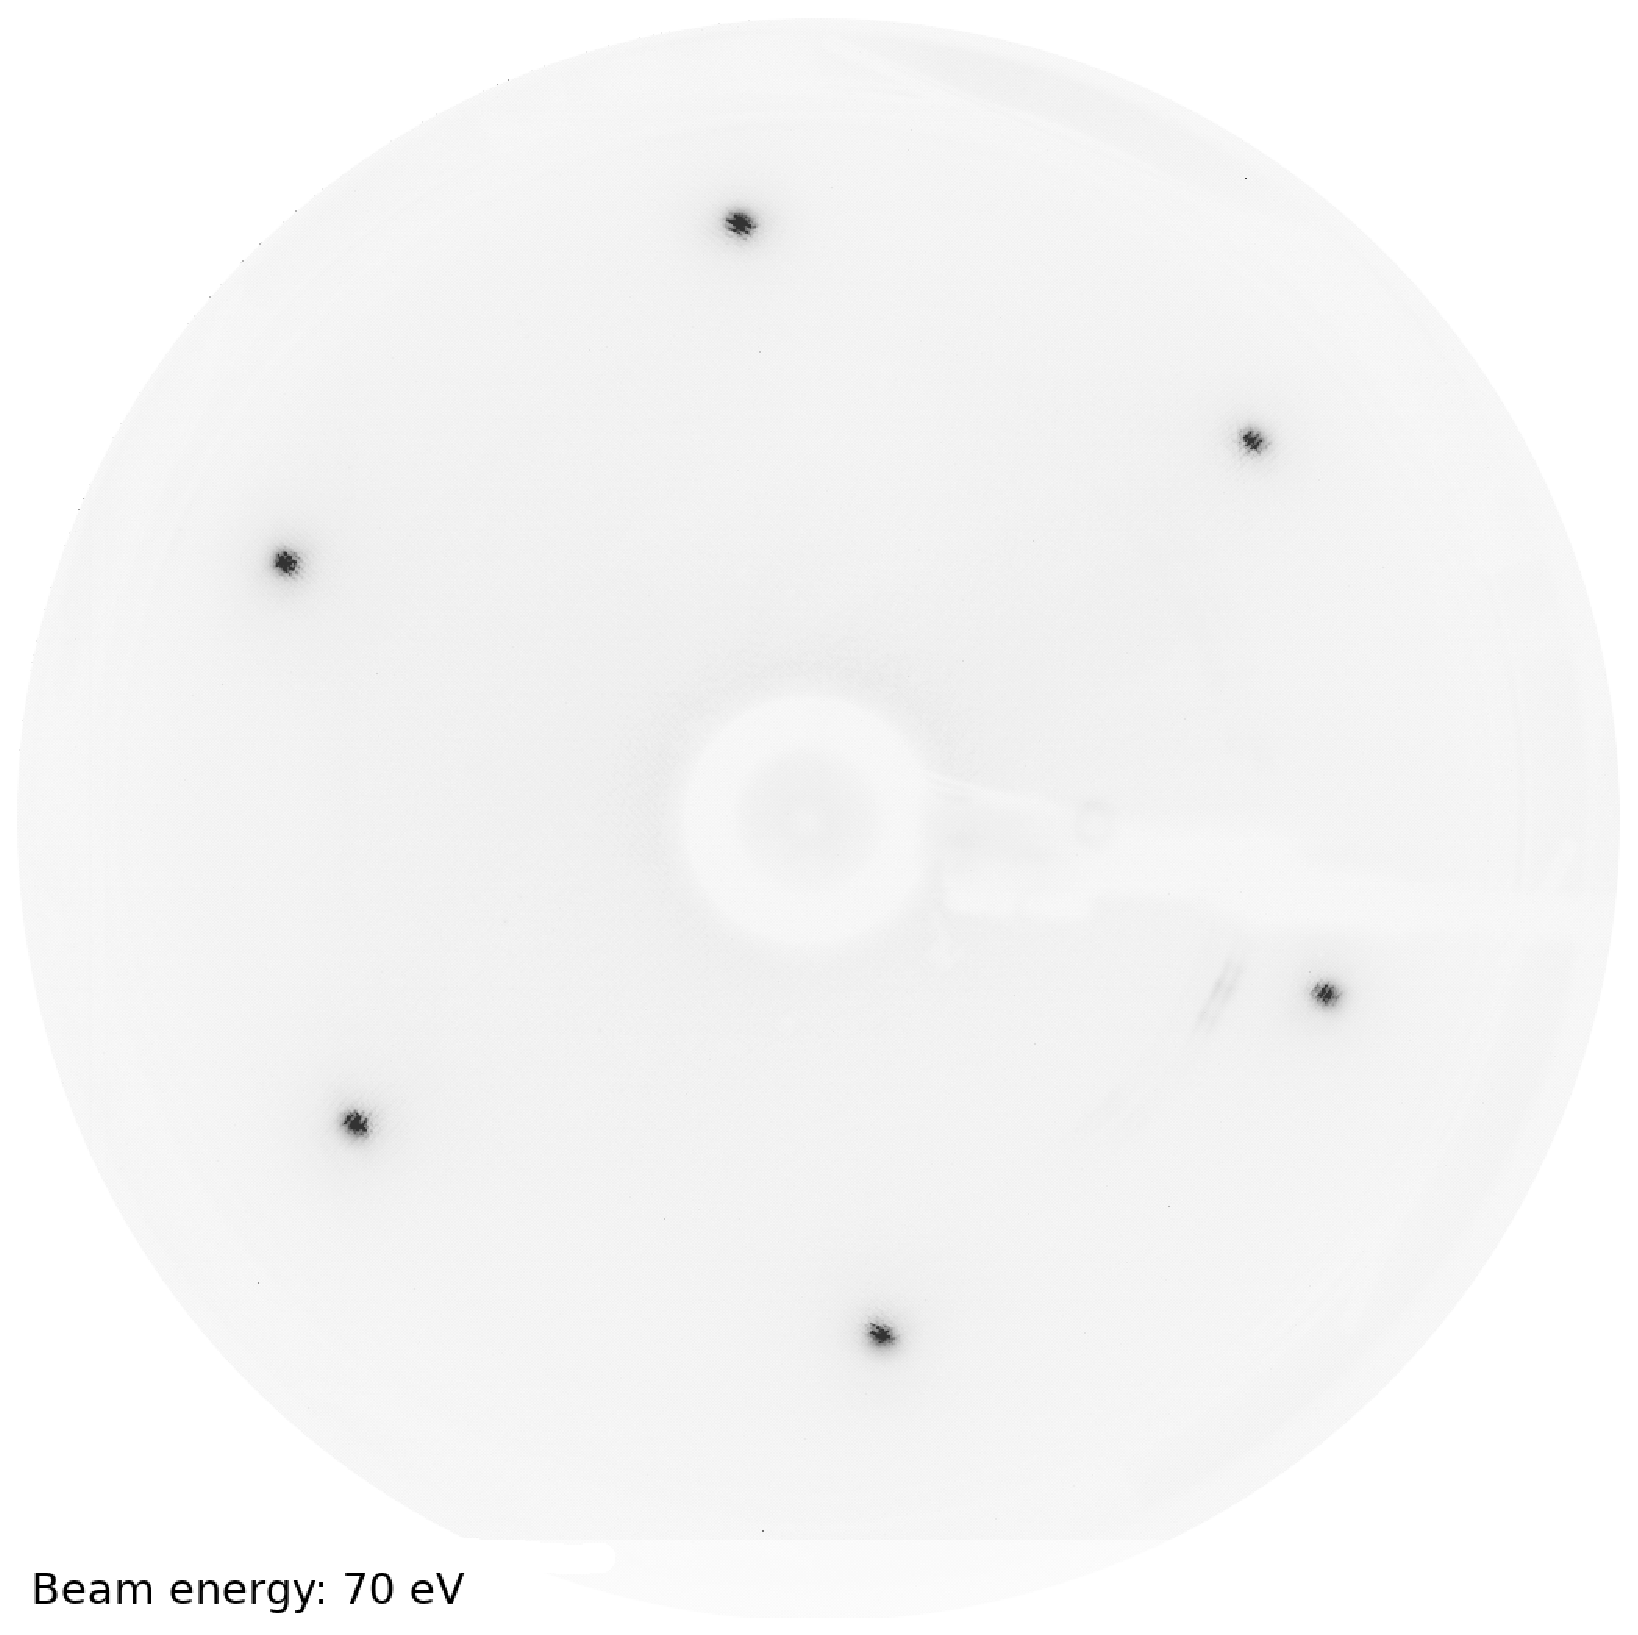
\includegraphics[width=0.3\linewidth]{LEED}}
\caption{LEED картина соответствующая поверхностной фазе h-BN/Co(0001)($E_p = 70 eV$).}
\label{pic:LEED}
\end{figure}
совпадают, поэтому монослой гексагонального нитрида бора ровно ложится на поверхность
кобальта и не образует структуру Муара.
Картина ДМЭ демонстрирует четко выраженную гексагональную структуру (1х1) рефлексов.
Это говорит о том, что выращенный кристалл h-BN имеет высокое качество, а также строго 
ориентирован относительно подложки.

\section{Экспериментальные спектры и их обсуждение}

Полученная конфигурация h-BN/Co(0001) была подвергнута окислению. Окисление проходило 
поэтапно, на каждом этапе производилось прогревание образца при температуре 300~$^\circ$C,
под давлением кислорода $10^{-5}$ мбар:
\begin{enumerate}
	\item Первый шаг. Окисление при давлении кислорода $10^{-5}$ мбар в течение 10 минут.
	\item Второй шаг. Окисление при давлении кислорода $10^{-5}$ мбар в течение 10 минут.
	\item Третий шаг. Окисление при давлении кислорода $10^{-5}$ мбар в течение 10 минут.
	\item Четвертый шаг. Окисление при давлении кислорода $10^{-5}$ мбар в течение 10 минут.
	\item Пятый шаг. Окисление при давлении кислорода $10^{-5}$ мбар в течение 10 минут.
	\item Шестой шаг. Окисление при давлении кислорода $10^{-5}$ мбар в течение 30 минут.
	\item Седьмой шаг. Окисление при давлении кислорода $10^{-5}$ мбар в течение 60 минут.
\end{enumerate}
Таким образом суммарное время окисления структуры составило 140 минут.
На каждом этапе снимались фотоэлектронные спектры(XPS) и спектры поглощения(NEXAFS).
Далее в работе представленны результаты обработки данных спектров.

\subsection{Спектры фотоэлектронной спектроскопии}

На рис.~\ref{pic:Surveys} представлена серия фотоэлектронных спектров поверхности h-BN/Co(0001).
Каждая кривая соответствует этапу окисления, таким образом, первая кривая характеризует
поверхность до окисления, а последняя после 140 минут. Видно, что вначале
\begin{figure}[!ht]
\center{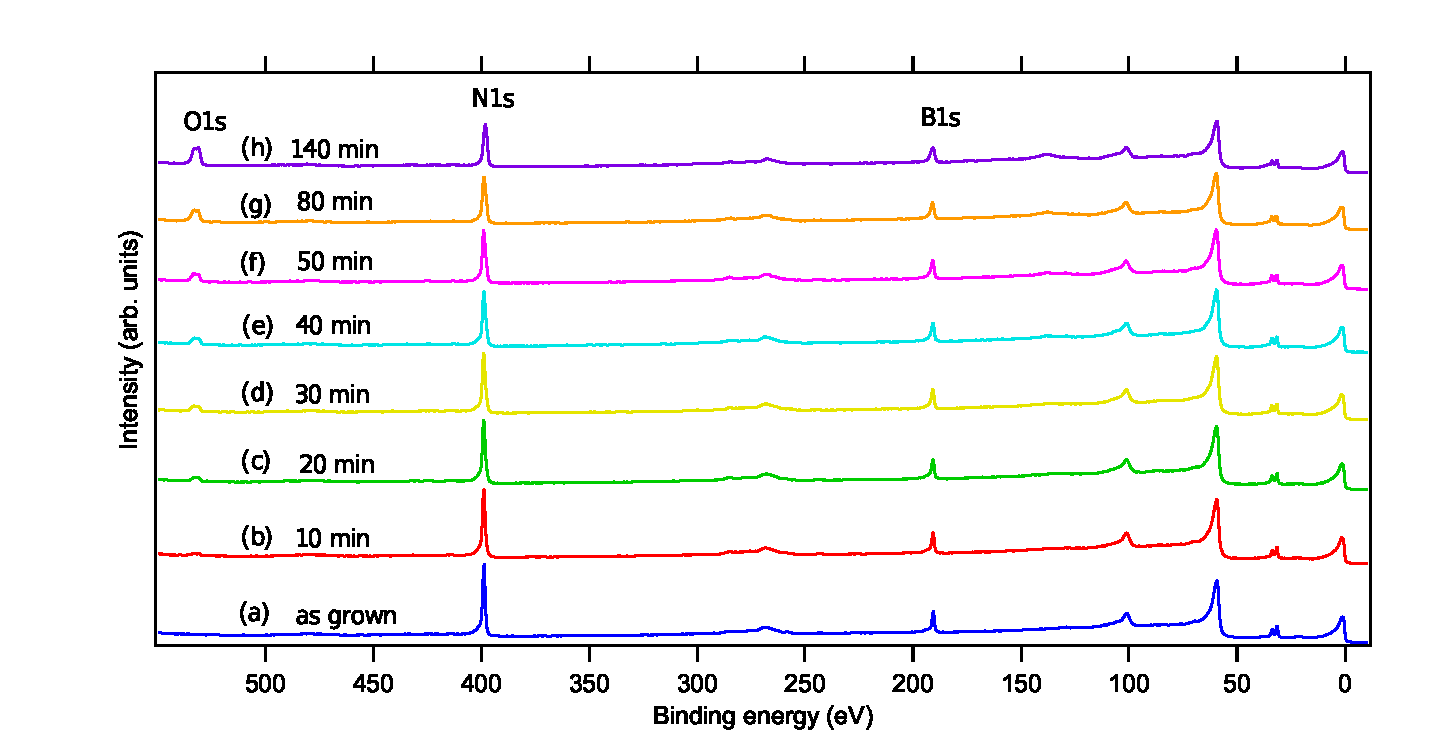
\includegraphics[width=1\linewidth]{Surveys}}
\caption{Обзорные фотоэлектронные спектры h-BN/Co(0001) в процессе окисления, записанные с энергией
возбуждающих квантов 650 eV}
\label{pic:Surveys}
\end{figure}
отсутствует пик кислорода O1s, который появляется уже на первом этапе после 10 минут 
окисления поверхности и растет со временем. Так же можно заметить, что интенсивность
пика азота N1s убывает в течение окисления, в то время, как интенсивность пика бора
B1s остается неизменной. Зависимость концентраций азота, бора и кислорода на поверхности
h-BN/Co(0001) от времени представлена на рис.~\ref{pic:B_N_O_tot_percent}. 
На чистой поверхности образца до окисления кислород отсутствует, а на бор с азотом приходится
по 50\% концентрации. Далее, с окислением поверхности, концентрация кислорода увеличивается
и доходит до отметки в 14.9\%. В процессе окисления концентрация азота уменьшается на 8.5\%.
Концентрация бора остается постоянной. Представленные зависимости демонстрируют, что количество 
азота в кристаллической решетке гексагонального нитрида бора убывает, а кислорода возрастает.
Такое же поведение системы h-BN/Ir(111) при окислении наблюдалось в работе~\cite{Simonov2012_h-BN/Ir_Oxydation}. 
\begin{figure}[!ht]
\center{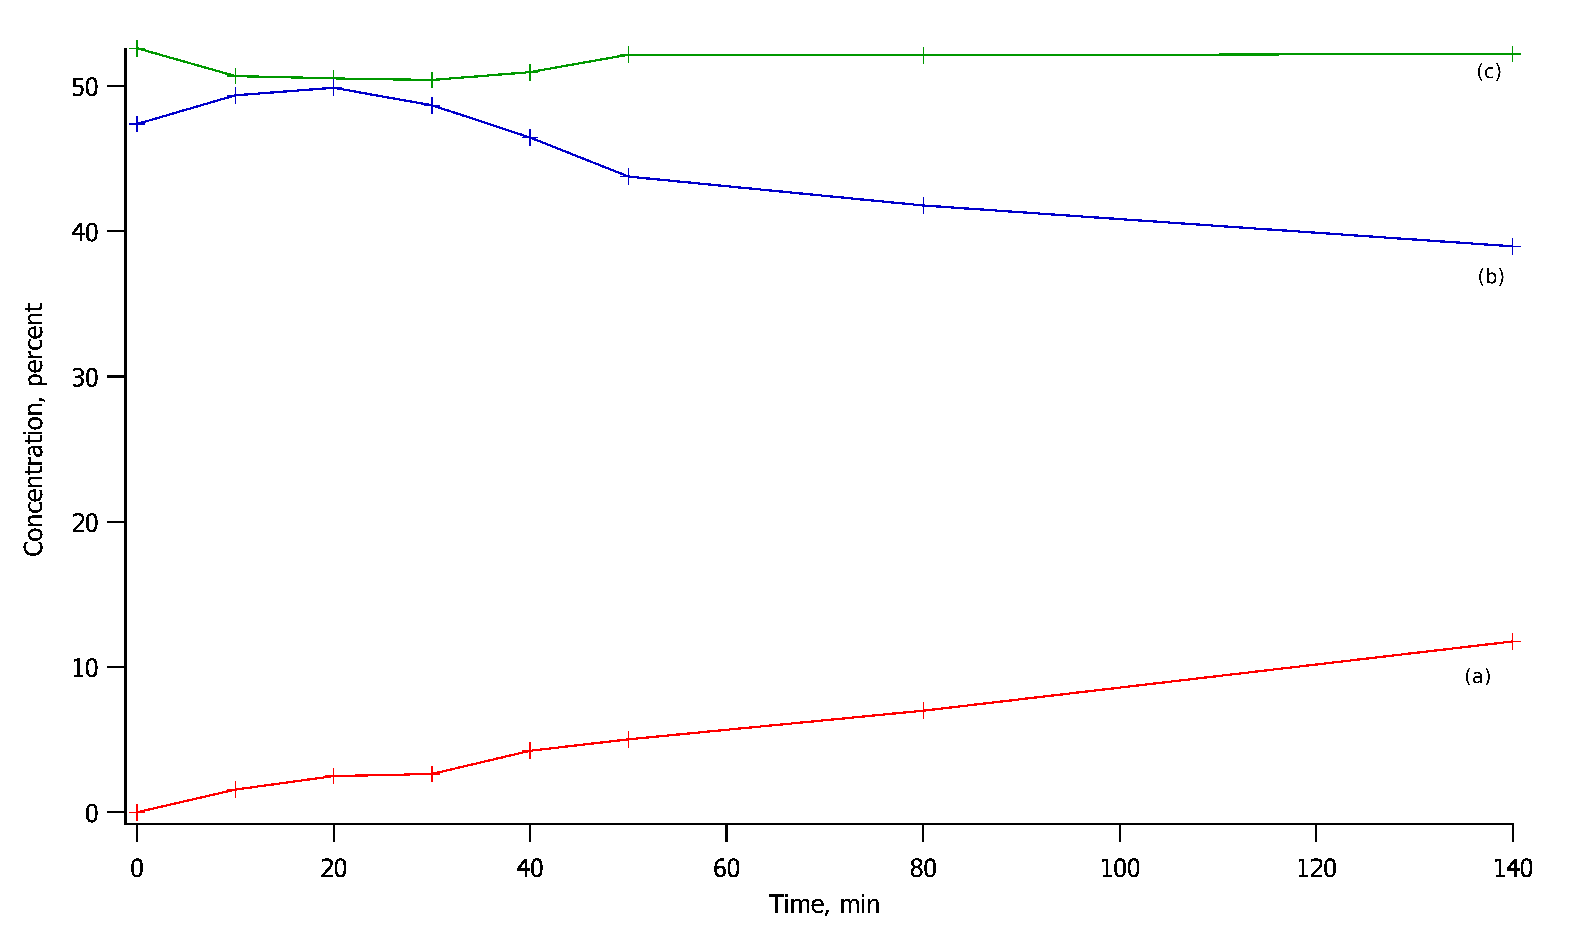
\includegraphics[width=0.8\linewidth]{N_B_O_tot_percent_vs_time}}
\caption{Зависимость концентраций от времени (a) бора, (b) азота, (c) кислорода.}
\label{pic:B_N_O_tot_percent}
\end{figure}
Здесь можно сделать предположение, что атомы кислорода встраиваются в кристаллическую решетку
нитрида бора, замещая атомы азота.


Далее мы рассмотрели пики интенсивностей B1s, N1s и O1s  в отдельности и пронаблюдали их эволюцию
от первого этапа с чистой поверхностью до последнего этапа после 140 минут окисления. 
На рис.~\ref{pic:B1s_N1s} представленны интенсивности фотоэмиссии пиков B1s и N1s.
\begin{figure}[!ht]
\center{\includegraphics[width=0.8\linewidth]{B1s_N1s_fits.eps}}
\caption{XPS линии (i) B1s-, (ii) N1s-уровней от исходного h-BN (as grown) и на разных стадиях окисления.}
\label{pic:B1s_N1s}
\end{figure}
Пик $\mathrm{b_1}$ на рисунке~\ref{pic:B1s_N1s}(i) с энергией связи 190.4 eV соответствует основному пику 
чистого h-BN сильно связанного с Co(0001). Уже после 10 минут окисления появляется два пика
$\mathrm{b_2}$ с энергией связи 191.3 eV и $\mathrm{b_3}$ с энергией связи 190.2 eV. Пик $\mathrm{b_3}$  имеет меньшую энергию связи,
чем $\mathrm{b_1}$ и появляется в результате интеркаляции кислорода под монослой нитрида бора. 
Энергия связи уменьшается, потому что атомы кислорода экранируют атомы бора от атомов кобальта. Пик $\mathrm{b_2}$ 
относительно $\mathrm{b_1}$ сдвинут в область больших энергий связи. Этот пик связан со встраиванием молекулярного кислорода
в решетку гексагонального нитрида бора, с замещением атома азота на атом кислорода, и образованием локальной структуры 
$\mathrm{BN_2O}$~\cite{Makarova2019_h-BN/Ni_Oxydation}. Кислород является более электроотрицательным, чем азот, поэтому энергия связи увеличивается.
Компонента $\mathrm{b_4}$ появляется только после 40 минут окисления и может
быть связана с образованием $\mathrm{BO_3}$, где уже все три атома азота замещены атомами кислорода, в следствии чего энергия связи
увеличивается еще сильнее. После 140 минут окисления пик $\mathrm{b_1}$ теряет свою интенсивность, а пики
$\mathrm{b_2}$ и $\mathrm{b_3}$ становятся преобладающими. Это говорит нам о том, что на поверхности h-BN при окислении
преимущественно образуются оксидные группы $\mathrm{BN_2O}$, а интеркаляция кислорода под монослой нитрида бора приводит
к ослаблению связи между монослоем h-BN и подложкой Co(0001).
\begin{figure}[!ht]
\center{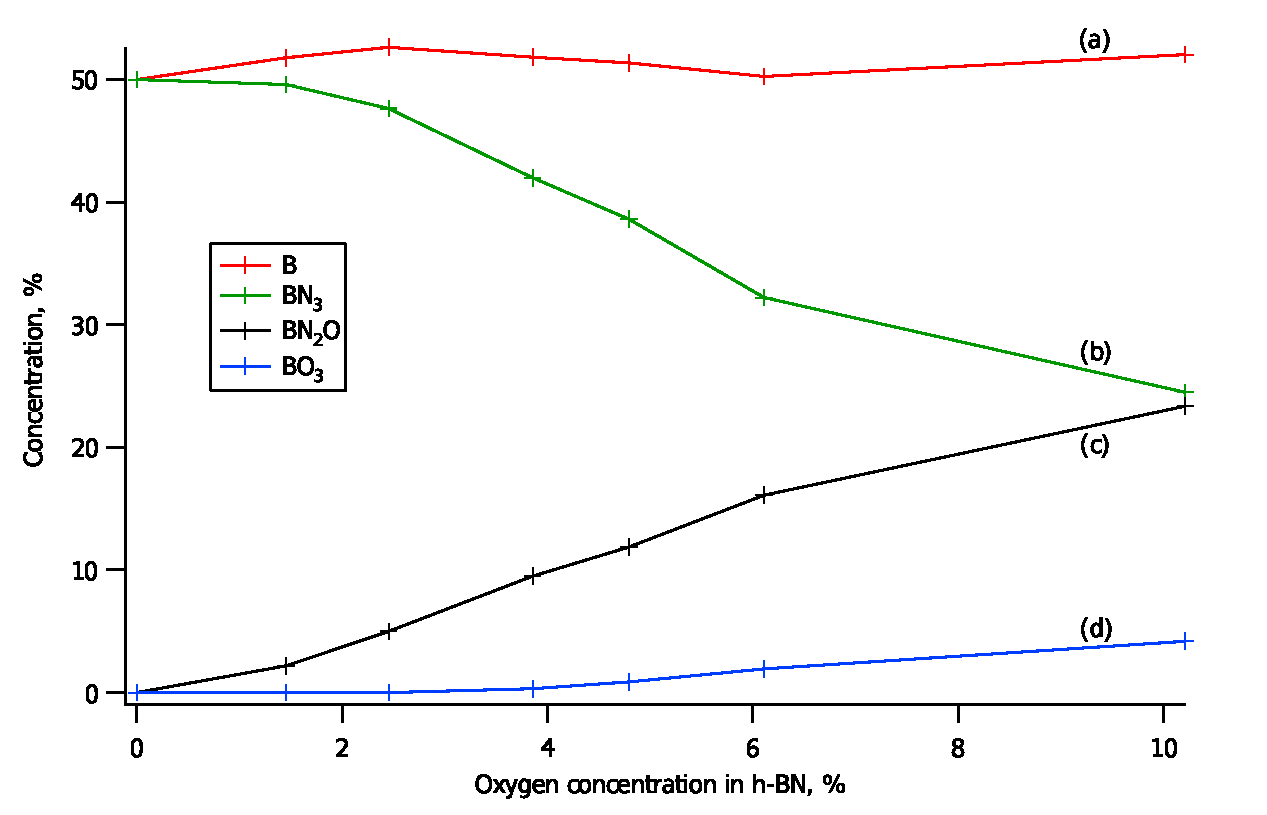
\includegraphics[width=0.8\linewidth]{Concentration_B_BN3_BN2O_BO3_vs_O.eps}}
\caption{График зависимости концентраций B (a), $\mathrm{BN_3}$ (b), $\mathrm{BN_2O}$ (c) и $\mathrm{BO_3}$ (d) от концентрации молекулярного кислорода, встроенного в решетку гексагонального нитрида бора.}
\label{pic:B_BN3_BN2O_BO3_vs_O}
\end{figure}


На рис.~\ref{pic:B_BN3_BN2O_BO3_vs_O} представлен график зависимости концентраций всего бора B (a), бора связанного с Co(0001)
$\mathrm{BN_3}$ (b), бора связанного с одним атомом кислорода $\mathrm{BN_2O}$ (c) и бора связанного с тремя атомами кислорода
$\mathrm{BO_3}$ (d) от концентрации молекулярного кислорода, встроенного в решетку гексагонального нитрида бора. Концентрация бора (d) на поверхности
остается неизменна на протяжении всего времени окисления. Концентрация бора сильно связанного с подложкой кобальта (b) характерно 
уменьшается и к седьмому этапу окисления с 50\% убывает до 24,5\%. Концентрация структуры $\mathrm{BN_2O}$, появляющейся уже после
первого этапа окисления, растет в течение всего эксперимента и к последнему этапу возрастает до 23.3\%. Структура $\mathrm{BO_3}$
появляется только после 40 минут окисления, а ее концентрация на последнем этапе доходит до отметки 4.1\%. Таким образом можно
сделать вывод, что с увеличением концентрации молекулярного кислорода в решетке h-BN, преимущественно образуются структуры вида
$\mathrm{BN_2O}$, при этом атомы бора не покидают решетку нитрида бора.


На рис.~\ref{pic:B1s_N1s}(ii) представлена серия фотоэмиссионных спектров азота N1s в течение окисления поверхности.
Пик $\mathrm{n_1}$ с энергией связи 398.5 соответствует основному пику чистого h-BN сильно связанного с Co(0001).
После 10 минут окисления в пике азота появляются две новые компоненты $\mathrm{n_2}$ с энергией связи 397.7 eV и
$\mathrm{n_3}$ с энергией связи 397.2 eV. Эти две компоненты связаны с интеркаляцией кислорода под монослой нитрида бора.
Интенсивность пика $\mathrm{n_1}$ со временем окисления заметно падает, в то время как пики $\mathrm{n_2}$ и $\mathrm{n_3}$
растут, и после 140 минут экспозиции все три пика $\mathrm{n_1}$, $\mathrm{n_2}$ и $\mathrm{n_3}$ оказываются примерно с
одинаковой интенсивностью. % Это говорит о том, что интеркаляция кислорода под монослой гексагонального нитрида бора экранирует
% его от подложки кобальта. Общая интенсивность пика N1s в течение окисления уменьшается, что является следствием того, 
% что количество азота в структуре h-BN/Co(0001) уменьшается, то есть замещенные кислородом атомы азота устраняются с поверхности.
\begin{figure}[!ht]
\center{\includegraphics[width=0.8\linewidth]{Conc_Nfree_Nco_Ntot_vs_O.eps}}
\caption{График зависимости концентраций всего азота (a), азота связанного с Co(0001) (b) и азота несвязанного с подложкой (b) и (с) от от концентрации кислорода, встроенного в решетку h-BN.}
\label{pic:Nfree_Nco_Ntot_vs_O}
\end{figure}


Зависимость концентраций пиков азота от концентрации молекулярного кислорода, встроенного в решетку гексагонального нитрида бора
представлена на рис.~\ref{pic:Nfree_Nco_Ntot_vs_O}. Кривая (a) соответствует концентрации азота на поверхности
h-BN/Co(0001). Убывание этой кривой свидетельствует о том, что количество азота в структуре h-BN/Co(0001) убывает в процессе
окисления. то есть замещенные кислородом атомы азота устраняются с поверхности. Азоту сильно связанному с Co(0001) соответствует 
кривая (b), она характерно убывает с ростом концентрации кислорода, в то время как кривые (c) и (d) быстро растут. Кривые (c) и (
d) отвечают азоту несвязанному с подложкой кобальта. Это атомы азота, под которые интеркалировали атомы кислорода. Такое поведение 
кривых концентраций говорит о том, что вместе с процессом встраивания молекулярного кислорода в решетку h-BN, так же происходит 
интеркаляция атомов кислорода под монослой гексагонального нитрида бора, и экранирование связи атомов азота и кобальта.


\begin{figure}[!ht]
\center{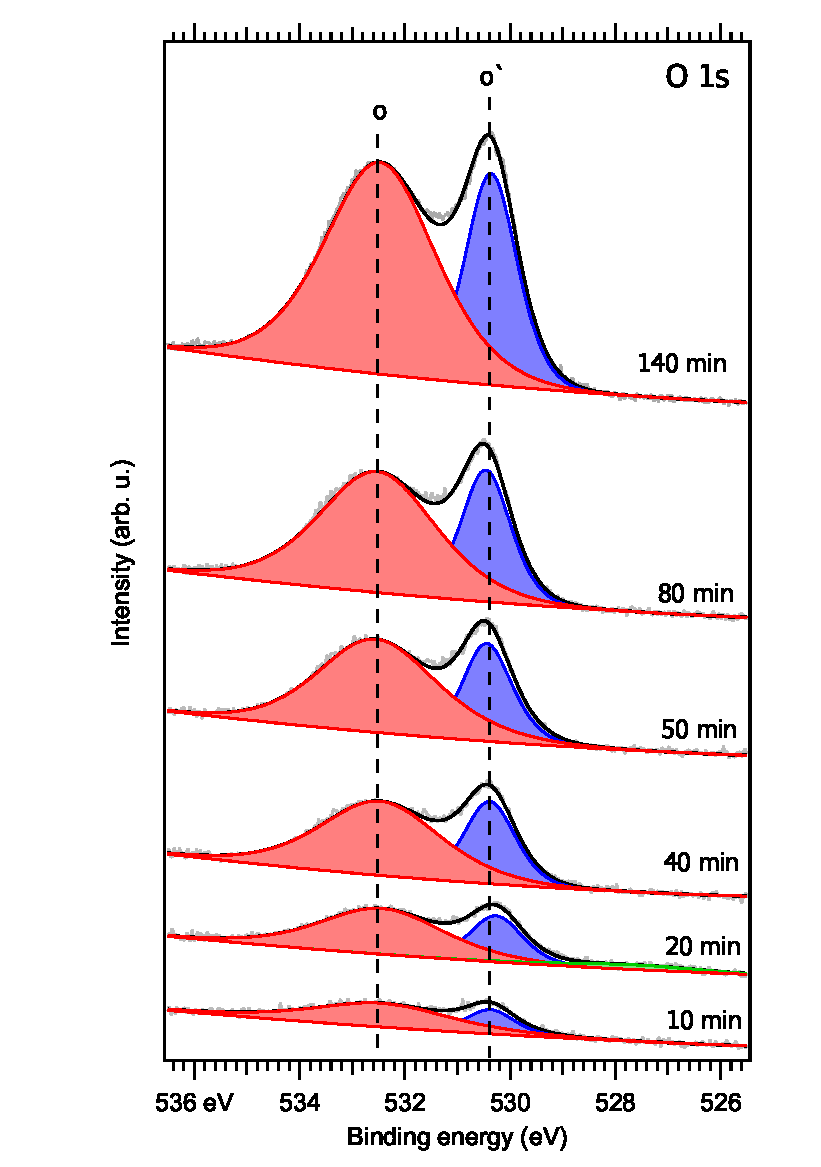
\includegraphics[width=0.5\linewidth]{O1s_all_fits.eps}}
\caption{XPS линии O1s-уровней на разных стадиях окисления.}
\label{pic:O1s_all}
\end{figure}
На рис.~\ref{pic:O1s_all} представлена серия спектров фотоэмиссии кислорода O1s в течение окисления поверхности.
Пик O1s содержит две компоненты: o с энергией связи 532.2 eV и o' с энергией связи 530.3 eV. Оба пика появляются
после 10 минут окисления и растут в течение всех этапов экспозиции. Пик о' относится к атомам кислорода, которые
интеркалировали под монослой нитрида бора. Пик о характеризует атомы кислорода, встроенные в решку h-BN в процессе
окисления. Большая ширина этого пика является следствием суперпозиции двух пиков оксидов $\mathrm{BN_2O}$ и
$\mathrm{BO_3}$~\cite{Shevelev2019_h-BN/Co_oxydation}. 


Далее на рис.~\ref{pic:O_components_vs_time} приведены зависимости компонент пика азота от времени. Кривая (а) соответствует кислороду 
встроенному в решетку нитрида бора, а кривая (b) это кислород интеркалированный под монослой h-BN. Видно,
что компонента встроенного кислорода растет быстрее интеркалированной. Значит кислород охотнее встраивается
в решетку монослоя, а не интеркалирует под него.
\begin{figure}[!ht]
\center{\includegraphics[width=0.6\linewidth]{O_components_vs_time.eps}}
\caption{Компонента встроенного (a) и интеркалированного (a) кислорода.}
\label{pic:O_components_vs_time}
\end{figure}


\subsection{Спектры поглощения NEXAFS}

Теперь рассмотрим спектры поглощения. После каждого этапа окисления вместе с фотоэмиссионными спектрами,
также снимались спектры поглощения NEXAFS. На рис.~\ref{pic:NEXAFS_B_K_edge} представлены B K-спектры
\begin{figure}[!ht]
\center{\includegraphics[width=0.8\linewidth]{BN_B_K_edge_all_40deg_to_beam.eps}}
\caption{Спектры поглощения B K-edge.}
\label{pic:NEXAFS_B_K_edge}
\end{figure}
поглощения h-BN, соответствующие исходному h-BN/Co(0001) (a), через 10 минут после экспозиции с кислородом (b), 
20 минут (c), 30 минут (d), 40 минут (e), 60 минут (d) и насыщенный кислородом h-BN/Co(0001), после 240 минут
экспозиции (f). Пик А соответствует гибридизированным состояниям h-BN-Co. В процессе окисления интенсивность
этого пика заметно понижается, и после 240 минут окисления пик А становится практически незаметным.
Пик B отвечает за квазисвободный гексагональный нитрид бора. Этот пик становится более острым в процессе 
окисления, это следствие интеркаляции молекулярного кислорода под монослой нитрида бора. Так же нельзя не 
обратить внимание на пики $\mathrm{a_1}$, $\mathrm{a_2}$ и $\mathrm{a_3}$ с энергиями связи 192.7 эВ, 193.3 эВ 
и 193.9 эВ соответственно. В работе \cite{Huber2015_Oxy_Stab_defffects_in_hBN} было показано, что пик $\mathrm{a_1}$
соответствует $\mathrm{BN_2O}$, пик $\mathrm{a_2}$ соответствует $\mathrm{BNO_2}$, а пик $\mathrm{a_3}$ соответствует
$\mathrm{BO_3}$. Исходя из интенсивностей пиков $\mathrm{a_1}$, $\mathrm{a_2}$ и $\mathrm{a_3}$, полученного спектра
поглощения B K- уровня, можно заключить, что на поверхности гексагонального нитрида бора при окислении преобладает
образование структуры $\mathrm{BN_2O}$, пик $\mathrm{a_1}$ в течение всего процесса окисления. После 240 минут окисления
так же становится явно выраженным пик $\mathrm{a_3}$, что говорит о появлении структуры $\mathrm{BO_3}$ на поверхности 
h-BN/Co(0001). Пик $\mathrm{a_2}$ становится заметным только после 240 минут окисления. Интенсивность этого пика очень
низкая, а значит структуры $\mathrm{BNO_2}$ практически не образовываются на поверхности гексагонального нитрида бора
при окислении в молекулярном кислороде.

\section{Моделирование окисленного нитрида бора}
\subsection{Статистический расчет окисления монослоя h-BN}
Для лучшего понимания процесса окисления гексагонального нитрида бора было выполнено моделирование окисленной системы 
h-BN исходя из предположения, что атомы кислорода встраиваются в решетку случайным образом. В процессе моделирования
была построена ячейка гексагонального нитрида бора 200х200, которая содержала 80000 атомов. Атомы азота случайным образом 
заменялись атомами кислорода. Количество атомов кислорода определялось из концентрации кислорода на поверхности в эксперименте. 
Далее были подсчитаны концентрации азота и структур вида $\mathrm{BN_3}$, $\mathrm{BN_2O}$, $\mathrm{BNO_2}$ и $\mathrm{BO_3}$ в 
кристаллической решетке  h-BN.
\begin{figure}[!ht]
\center{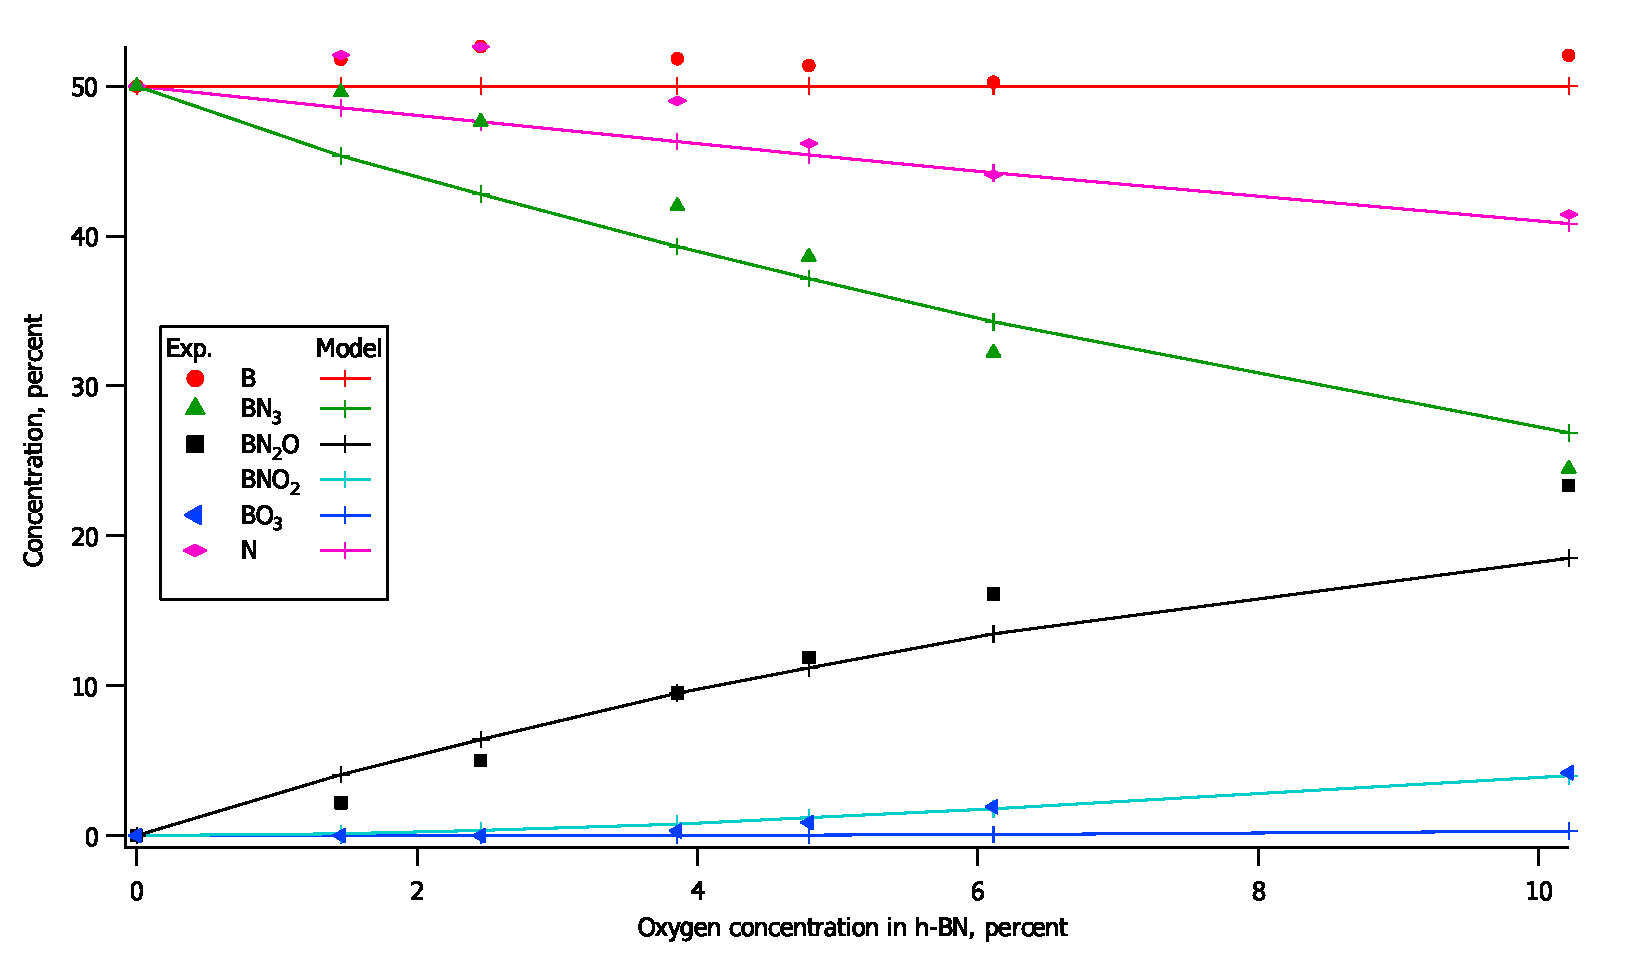
\includegraphics[width=0.8\linewidth]{BN_200x200_experiment_and_model.eps}}
\caption{Экспериментальные и статистически рассчитанные концентрации азота и бора в зависимости от концентрации кислорода 
в решетке h-BN.}
\label{pic:BN_200x200_experiment_and_model}
\end{figure}
На рис.~\ref{pic:BN_200x200_experiment_and_model} представлены для сравнения экспериментальные и статистически 
рассчитанные концентрации азота и бора в зависимости от концентрации кислорода в решетке h-BN. Из графика видно,
что все модельные кривые концентраций, кроме $\mathrm{BNO_2}$ и $\mathrm{BO_3}$, согласуются с экспериментально полученными 
концентрациями. Из расчета получается, что количество образованных структур  $\mathrm{BNO_2}$ в течение окисления
преобладает над структурами $\mathrm{BO_3}$, что отражено на рис.~\ref{pic:BN_200x200_experiment_and_model}. Однако
в эксперименте, как было сказано ранее, структуры вида $\mathrm{BNO_2}$ практически не образовывались на поверхности.
На графике видно, что экспериментальная кривая $\mathrm{BO_3}$ совпадает с модельной кривой $\mathrm{BNO_2}$. Отсюда
можно сделать вывод, что в реальном эксперименте структуры $\mathrm{BNO_2}$ практически не образуются, вместо них
сразу появляются структуры $\mathrm{BO_3}$. 

\subsection{Расчет структуры \textbf{$\mathrm{BNO_2}$}}
Чтобы понять почему структуры вида $\mathrm{BNO_2}$ не образуются в эксперименте, с помощью DFT в программе
FPLO(Full-Potential Local-Orbital)~\cite{Koepernik1999} была рассчитана такая структура. Для этого рассмотрена ячейка гексагонального 
нитрида бора в вакууме. Ячейка содержала встроенные атомы кислорода таким образом, что они образовывали структуру
$\mathrm{BNO_2}$. Релаксация такой системы показала, что структура $\mathrm{BNO_2}$ является неустойчивой. 
\begin{figure}[!ht]
\begin{minipage}[h]{0.49\linewidth}
\center{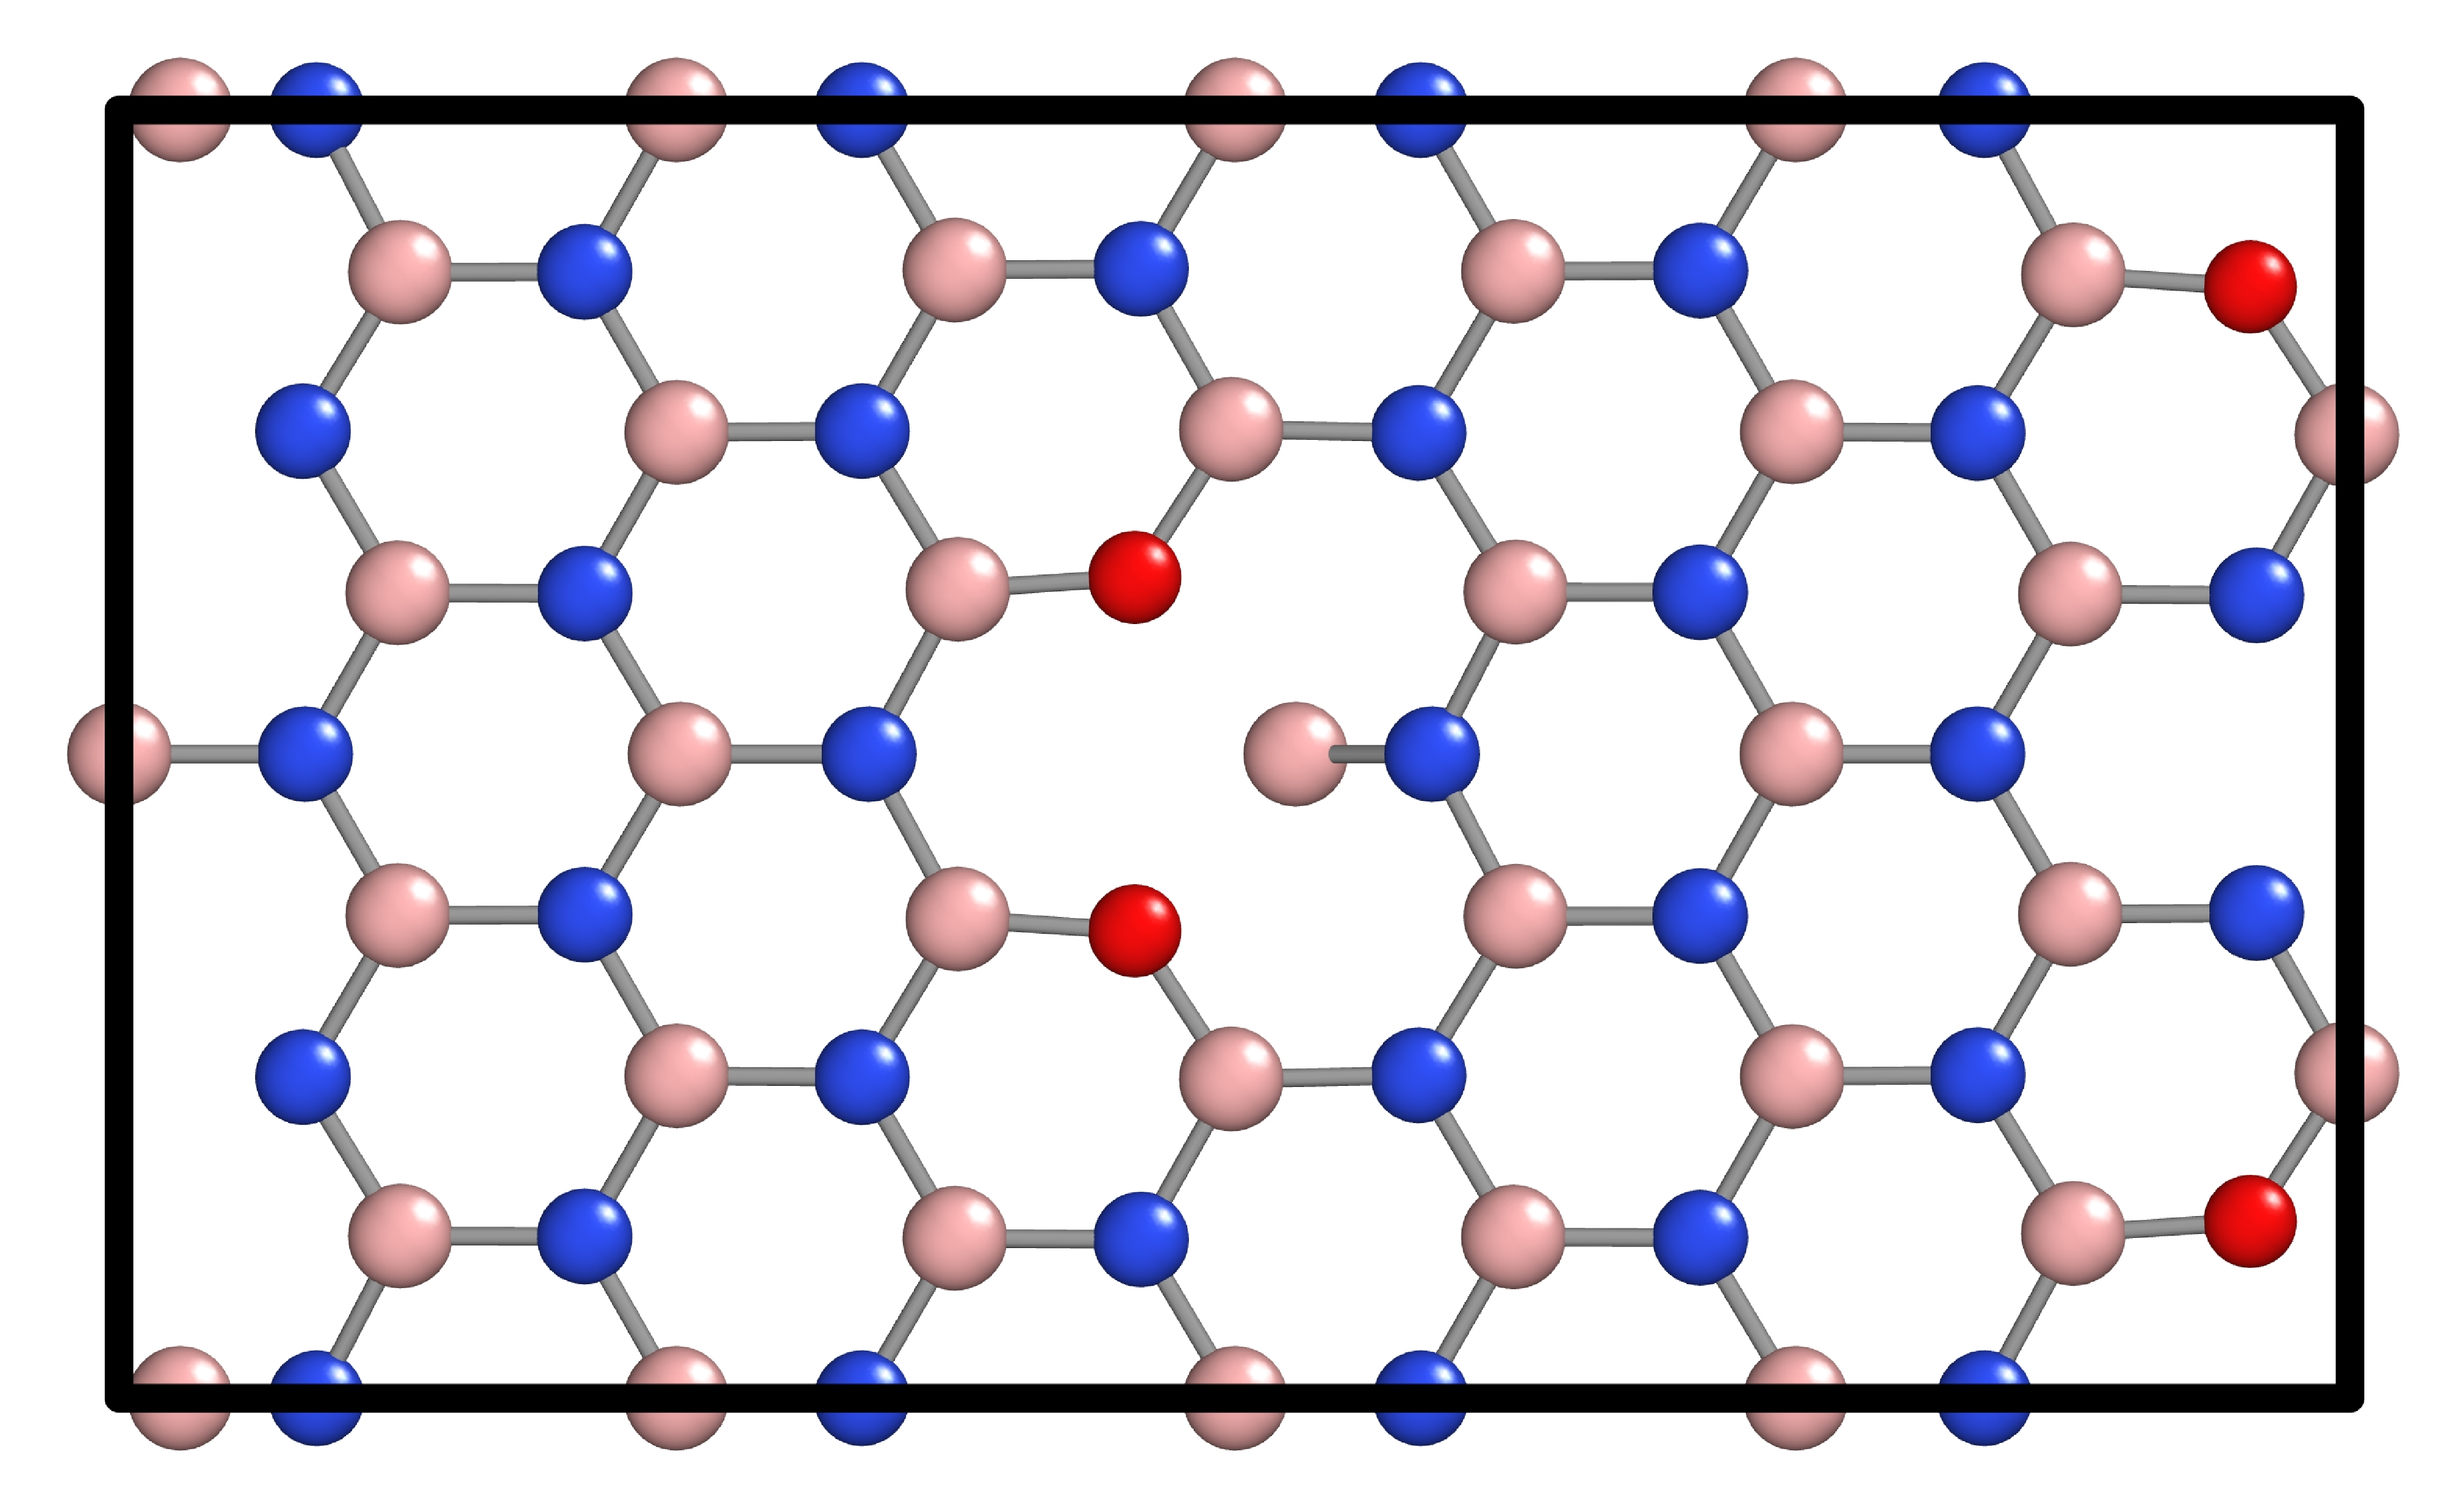
\includegraphics[width=0.9\linewidth]{BNO2_relaxed3.eps} \\ а)}
\end{minipage}
\hfill
\begin{minipage}[!ht]{0.49\linewidth}
\center{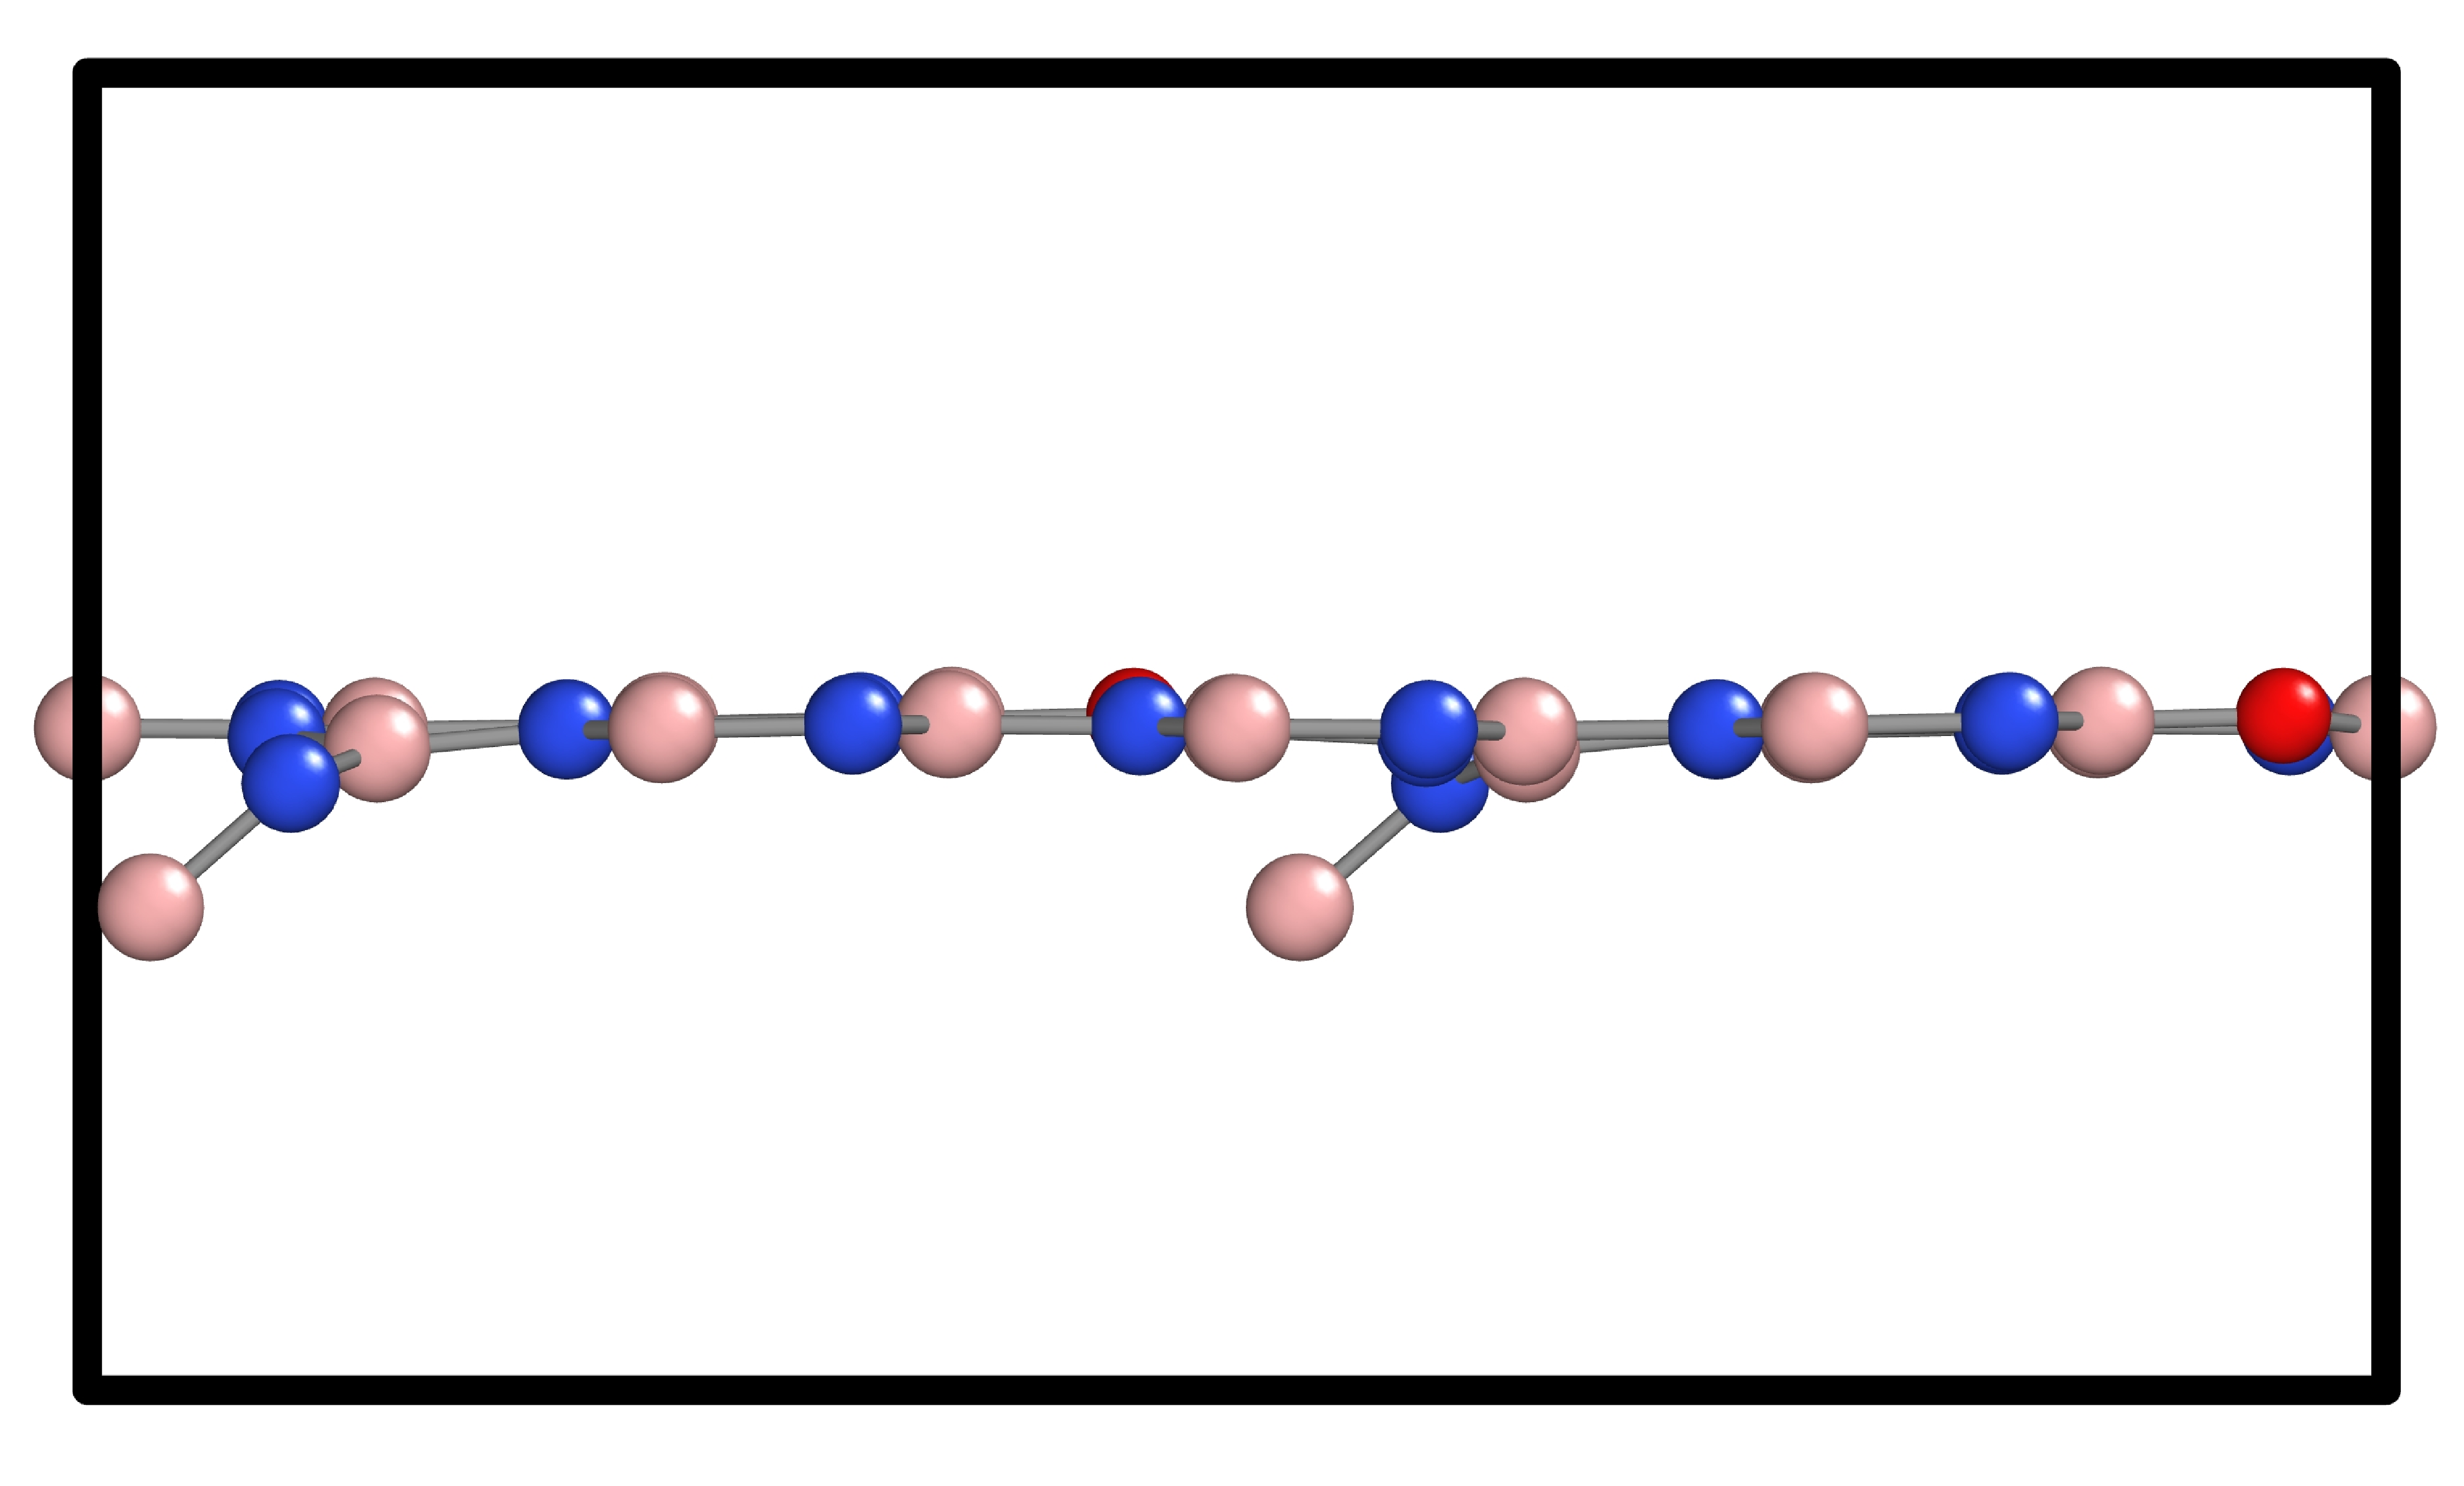
\includegraphics[width=0.9\linewidth]{BNO2_relaxed4.eps} \\ б)}
\end{minipage}
\caption{$\mathrm{BNO_2}$ в кристаллической решетке h-BN.}
\label{BNO2_relaxed}
\end{figure}
На рис.~\ref{BNO2_relaxed} приведена рассчитанная методом DFT кристаллическая решетка гексагонального нитрида бора 
со встроенными атомами кислорода. Видно, что атомы кислорода выдавливают атомы бора из решетки h-BN, в результате чего
последние оказываются несвязанными с решеткой. Расстояние от выдавленного кислородами  атома бора до монослоя h-BN
достигает 1.44~\AA, это проиллюстрировано на рис.~\ref{pic:BNO2_B_height}. Этот расчет говорит о том, что структуры
вида $\mathrm{BNO_2}$ оказываются нестабильными и энергетически не выгодными. Это и является причиной отсутствия 
$\mathrm{BNO_2}$ в эксперименте.
\begin{figure}[!ht]
\center{\includegraphics[width=0.6\linewidth]{BNO2_B_height.png}}
\caption{Рассчитанная методом DFT структура $\mathrm{BNO_2}$.}
\label{pic:BNO2_B_height}
\end{figure}



\clearpage
